\section{\texorpdfstring{Návrh dekodéru}{Navrh dekoderu}}

% =====================================================================================================================
	\begin{frame}
    \frametitle{Zadání}
		\boldmath
		Navrhujeme dekodér segmentu \textbf{f} 7-segmentového displeje.
		
		\begin{center}
			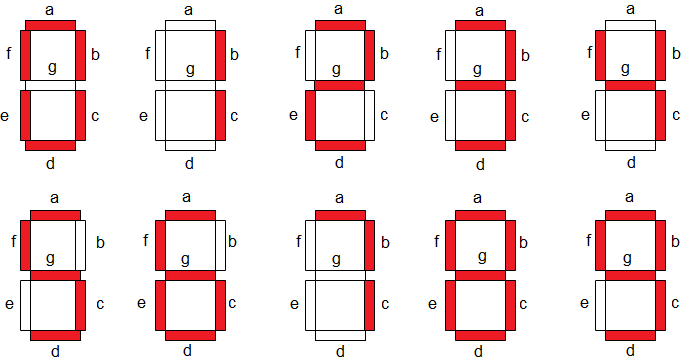
\includegraphics[width=1.00\textwidth]{fig/Seven-segment-display.png}
		\end{center}
		
	\end{frame}
	
% =====================================================================================================================
	\begin{frame}
    \frametitle{Pravdivostní tabulka}
		\boldmath
		
		\begin{minipage}[t][0.7\textheight][t]{0.45\textwidth}
		\vspace{5mm}
		
		První polovina
		\begin{center}
			\begin{tabular}{ c c c c | c }
				$A$ & $B$ & $C$ & $D$ & $Y$\\
				\hline
				0 & 0 & 0 & 0 & 1 \\
				0 & 0 & 0 & 1 & 0 \\
				0 & 0 & 1 & 0 & 0\\
				0 & 0 & 1 & 1 & 0\\
				0 & 1 & 0 & 0 & 1 \\
				0 & 1 & 0 & 1 & 1 \\
				0 & 1 & 1 & 0 & 1 \\
				0 & 1 & 1 & 1 & 0 \\
			\end{tabular}
		\end{center}

		\end{minipage}
		\begin{minipage}[t][0.7\textheight][t]{0.45\textwidth}
    \vspace{5mm}
		
		Druhá polovina
		\begin{center}
			\begin{tabular}{ c c c c | c }
				$A$ & $B$ & $C$ & $D$ & $Y$\\
				\hline
				1 & 0 & 0 & 0 & 1 \\
				1 & 0 & 0 & 1 & 1 \\
			  1 & 0 & 1 & 0 & x \\
				1 & 0 & 1 & 1 & x \\
				1 & 1 & 0 & 0 & x \\
				1 & 1 & 0 & 1 & x \\
				1 & 1 & 1 & 0 & x \\
				1 & 1 & 1 & 1 & x \\
			\end{tabular}
		\end{center}
		\end{minipage}
		
		Stavy \textbf{x} si zvolím až podle minimalizace v mapě.
	\end{frame}
	
% =====================================================================================================================
	\begin{frame}
    \frametitle{Karnaughova mapa - minimalizace}
		\boldmath
		\begin{center}
		  \begin{karnaugh-map}[4][4][1][$B$][$C$][$A$][$D$]
				\minterms{0,1,3,4,12,9}
				\implicant{0}{5}
				\implicant{4}{14}
				\implicant{1}{9}
				\implicant{1}{7}
				\indeterminants{5,6,7,13,14,15}
				
				% ====== vlastní čáry ======

				% A = 1 (řádek 2 a 3)
				\draw[very thick] (-0.15,1) -- (-0.15,3);

				% B = 1 (sloupce 3 a 4)
				\draw[very thick] (2,4.3) -- (4,4.3);

				% C = 1 (sloupce 2 a 3)
				\draw[very thick] (1,4.15) -- (3,4.15);
				
				% A = 1 (řádek 3 a 4)
				\draw[very thick] (-0.30,0) -- (-0.30,2);

			\end{karnaugh-map}
			
		$Y = \textcolor{red}{\bar{C}\bar{D}} + \textcolor{green}{A} + \textcolor{orange}{B\bar{C}} + \textcolor{blue}{B\bar{D}}$
		\end{center}
	\end{frame}

% =====================================================================================================================
	\begin{frame}
    \frametitle{Úprava rovnice}
		\boldmath
		
		Obvod realizujeme pomocí hradel \textbf{NAND}:
		\begin{align*}
      Y =& \bar{C}\bar{D} + A +  B\bar{C} + B\bar{D} = \bar{\bar{Y}} = \\
				=& \overline{\overline{\bar{C}\bar{D} + A +  B\bar{C} + B\bar{D}}} \\
				=& \overline{\overline{\bar{C}\bar{D}} \cdot \bar{A} \cdot \overline{B\bar{C}} \cdot \overline{B\bar{D}}}
		\end{align*}
		
		Při pohledu zdola nahoru na výsledný vztah, mi jednotlivé negace již ukazují, jak bude obvod zapojen. 
	\end{frame}

% =====================================================================================================================
	\begin{frame}
    \frametitle{Výsledek}
		\boldmath
		Obvod v logisim:
		
		\begin{center}
			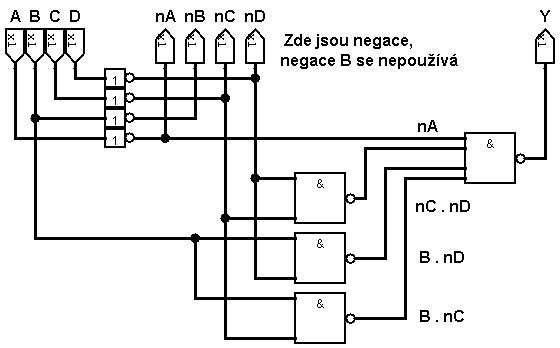
\includegraphics[width=0.90\textwidth]{fig/dekoder_obvod.png}
		\end{center}
		
	\end{frame}